\subsection{Desarrollo teórico}
Para comenzar el desarrollo teórico, primero definiremos la geometría de la bobina de manera esquemática para entender bien el sistema con el que trabajamos. De manera descriptiva, lo que tenemos es un cilindro hueco de radio \( r_{cint} \) y altura \( h_c \) sobre el cual enrollaremos un hilo de cobre \textbf{\textit{N}} veces, resultando en un radio exterior \( r_{cext} \). Ligeramente introducido en el cilindro hueco, se encuentra el vástago, que es un cilindro de acero (REFERENCIAR EL ACERO BIEN) de radio \( r_b \) y longitud \( L_b \). La corriente de alimentación será \( i_{dc} \). En la siguiente figura se resume todo en un esquema:

\begin{figure}[h]
    \centering
    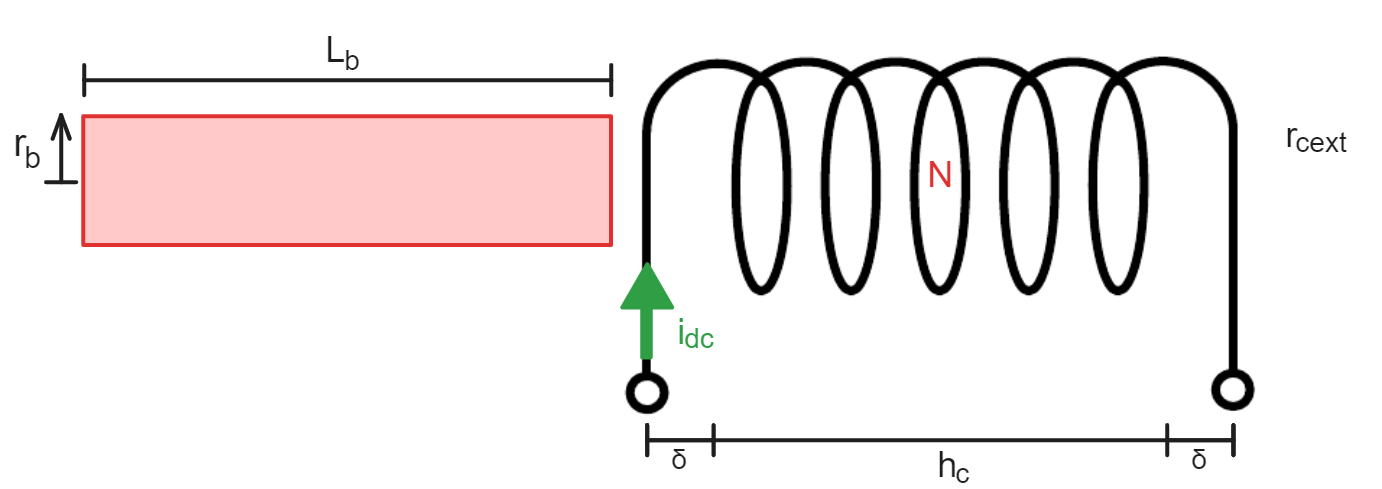
\includegraphics[width=\linewidth]{FigurasMemoria/fig1esquemaGeom.png}
    \caption{Esquema de la bobina y el vástago con sus dimensiones geometrías. Elaboración propia.}
    \label{fig:1} %Para referenciar -> \ref{fig:figNum}
\end{figure}

Para poder obtener valores númericos, vamos a considerar los siguientes datos geométricos de una bobina física con la que serán realizadas las pruebas y validaciones.

\[
L_b=0.096m~~~~r_b=0.003045m
\\~\\
h_c=0.05321m~~~~\delta=0.15*h_c~~~~r_{cext}=0.01064m
\\~\\
i_{dc}=3.5A~~N=500
\]

Para empezar el desarrollo, partiremos de la ley integral de Àmpere:

\[
Ni=\oint{\vec{H}\vec{dl}}
\]

Asumiendo un flujo uniforme en la bobina, podemos reescribir:

\[
Ni=Hh_c\to H=\frac{Ni_{dc}}{h_c}
\]

Buscamos ahora una expresión para la densidad de flujo:

\[
B=\mu_0\mu_r H=\mu_0\mu_r\frac{Ni_{dc}}{h_c}
\]